\chapter{SafeWatch: Sistema de Detecção de Quedas}
\label{cap:safeWatch}

Neste trabalho, apresentamos o SafeWatch, uma solução integrada entre smartphone e smartwatch, onde quedas são detectadas de maneira automatizada através de um algoritmo de detecção baseado em limiares. Quando necessário, os contatos de emergência do idoso são informados de sua localização para que possa prestar socorro de forma mais rápida possível. 

As seções desse capítulo são organizadas da seguinte maneira: A Seção \ref{sec:architecture} mostra a arquitetura que foi definida e utilizada pela ferramenta construída; A Seção \ref{sec:tools} mostra as ferramentas que foram utilizadas para auxiliar à construção do SafeWatch; Já a Seção \ref{sec:implementation} descreve detalhes da implementação do SafeWatch.



\section{Arquitetura}
\label{sec:architecture}

De acordo com \cite{garlan1993introduction}, a arquitetura de um software define o sistema em termos de componentes e as interações existentes entre esses componentes. Em outras palavras, a arquitetura de software tem o objetivo de mostrar uma visão geral do sistema. 

O SafeWatch foi desenvolvido para funcionar como um aplicativo Android Wear\footnote{https://www.android.com/wear/} para smartwatches que funciona em conjunto com o smartphone Android do usuário, através de uma aplicação homônima, que está sincronizada com o mesmo.

De forma geral, a aplicação smartwatch irá monitorar as atividades do usuário através do acelerômetro e no momento em que uma queda for detectada emitirá um alerta vibratório juntamente com um sinal para o smartphone. No smartphone está presente uma aplicação de gerenciamento geral do sistema, onde o usuário é capaz de adicionar, visualizar e remover os contatos de emergência que seriam notificados no momento de uma queda. Na ocorrência de uma queda o sistema irá se comportar como pode ser visto na Figura \ref{fig:diagram}.

\begin{figure}[ht]
	\centering
	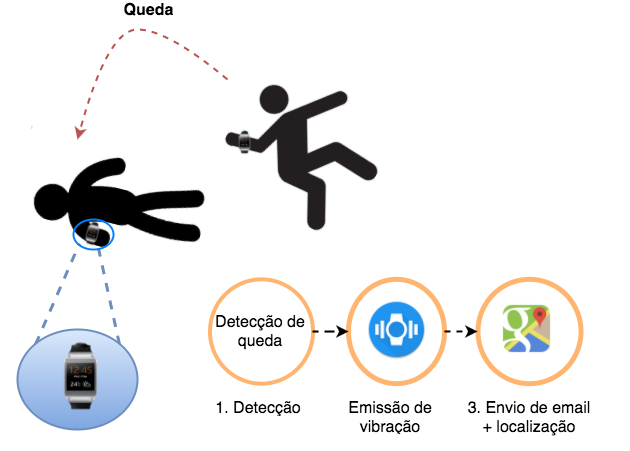
\includegraphics[scale=0.5]{imagens/DiagramaQueda.png}
	\caption{Aplicação no evento de queda. Figura Elaborada pelo autor (2016).}
	\label{fig:diagram}
\end{figure}



Assim que um evento de queda é detectado, o smartwatch irá emitir um sinal de vibração por um tempo determinado, e caso o usuário não informe o contrário, um email contendo a localização do usuário que está utilizando o smartwatch é enviado para os seus contatos de emergência previamente cadastrados.

O SafeWatch foi desenvolvido com base em uma arquitetura pré-definida e possui os seus módulos desacoplados para facilitar futuras mudanças ou melhorias. Na Figura \ref{fig:architecture} é possível ver o fluxo de dados dos cinco módulos presentes no SafeWatch. O fluxo começa com a obtenção dos dados do acelerômetro e termina com envio da mensagem de emergência. As setas na imagem representam o sentido do fluxo dos dados. Os módulos utilizados são os seguintes:


 \begin{figure}
 	\centering
 	\includegraphics[scale=0.65]{imagens/architecture.png}
 	\caption{ Fluxo de Dados do SafeWatch. Figura Elaborada pelo autor (2016).}
 	\label{fig:architecture}
 \end{figure} 


\begin{enumerate}
	\item{\textbf{Sensor Reader}: Responsável pela configuração e gerenciamento dos sensores, mais especificamente do sensor utilizado, o acelerômetro. }
	
	\item{\textbf{Fall Detector}: Recebe informações provindas do \textit{Sensor Reader} para através do algoritmo de detecção de quedas categorizar um determinado evento como queda ou não.}
	
	\item{\textbf{Watch Communicator}: Realiza a comunicação entre o smartwatch e o smartphone do usuário. Irá receber dados do smartwatch que são tratados pelo módulo chamado de \textit{Fall Handler}.}
	
	\item{\textbf{Fall Handler}: Será responsável pelas ações do smartphone após um evento de queda, como o envio de emails e o gerenciamento dos dados do acelerômetro recebidos do smartwatch.}
	
	\item{\textbf{Contact Manager}: Será responsável pelo gerenciamento dos contatos de emergência do usuário. Ações como visualização, adição e remoção de contatos estão encapsuladas neste módulo.}
			
\end{enumerate}

Os módulos \textit{Sensor Reader} e \textit{Fall Detector} estão presentes na aplicação embarcada no smartwatch, os demais módulos estão presentes na aplicação para smartphones. 



\section{Ferramentas Utilizadas}
\label{sec:tools}
Durante o desenvolvimento do \textit{SafeWatch} foram utilizadas diversas ferramentas que serviram para dar suporte a sua implementação e execução. Tanto o aplicativo para smartphones, quanto o aplicativo embarcado no smartwatch foram desenvolvidos utilizando o Android Studio\footnote{https://developer.android.com/studio/}. O Android Studio é a \ac{IDE} oficial do Google no desenvolvimento de aplicações móveis ou vestíveis.


Nas classes do projeto relacionadas às telas do aplicativo foi utilizado o ButterKnife\footnote{texthttps://github.com/JakeWharton/butterknife}. O ButterKnife é responsável por fazer a ligação entre os arquivos responsáveis pela criação das telas, e as classes que utilizam os componentes visuais destas telas. 

Para realizar os cálculos do desvio-padrão foi utilizada a biblioteca do Apache chamada Commons-Math\footnote{http://commons.apache.org/proper/commons-math/}. Esta biblioteca contém um conjunto de funções matemáticas e de estatística não presentes na biblioteca padrão do JAVA. 

Para que possamos enviar os dados do acelerômetro do smartwatch para o smartphone, eles precisam estar codificados em algum padrão, o padrão escolhido foi o JSON. O JSON é um formato de dados utilizado para comunicação entre dispositivos \citep{JSON16}. Para que possamos fazer a codificação e decodificação dos dados do acelerômetro foi utilizada a biblioteca chamada Gson\footnote{http://www.json.org/}.

Por fim, para o envio de emails para os contatos de emergência foi utilizada a biblioteca padrão criada pela Oracle\footnote{http://www.oracle.com/} chamada de JavaMail\footnote{http://www.oracle.com/technetwork/java/javamail/index.html}. 





\section{Implementação}
\label{sec:implementation}
A implementação do SafeWatch foi dividida em várias partes, onde cada uma delas é representada por um módulo independente dos demais. A linguagem de programação utilizada foi Java\footnote{http://www.oracle.com/technetwork/java/index.html}, linguagem padrão no desenvolvimento de aplicações Android. Nas seções a seguir são detalhados detalhes da implementação e funcionamento de cada módulo.


\subsection{Sensor Reader}
O módulo \textit{Sensor Reader} é responsável pela configuração e gerenciamento do acelerômetro. Aqui, o acelerômetro é configurado para atualizar seus dados a uma frequência de 50 $Hz$, ou seja, a cada 20 ms. Os dados do acelerômetro são coletados a todo momento, mesmo quando a aplicação não está em primeiro plano.

Este módulo também será responsável por armazenar os dados do acelerômetro nos últimos 0.4 segundos para posterior uso no algoritmo de detecção, caso necessário. Tanto a escolha da frequência de 50 $Hz$ quanto o tempo de 0.4 segundos para o armazenamento de dados do acelerômetro serão explicados com mais detalhes na Seção \ref{subsec:fall_detector}. 


\subsection{Fall Detector}
\label{subsec:fall_detector}
O módulo \textit{Fall Detector} encapsula o algoritmo de detecção de quedas baseado em limiares utilizado pelo SafeWatch. Este é o módulo mais complexo da aplicação, pois nele se encontra a lógica responsável por decidir, através dos dados obtidos do acelerômetro, se um evento de queda ocorreu ou não. O algoritmo proposto é uma adaptação do algoritmo desenvolvido por \cite{hsieh2014wrist}. 

O algoritmo proposto neste trabalho se diferencia do algoritmo proposto em \cite{hsieh2014wrist} pela não utilização do giroscópio como sensor auxiliar, pois acredita-se que sem o uso desse sensor é possível obter-se resultados satisfatórios, como visto na Seção \ref{subsec:hsieh}, reduzindo o custo de bateria. O giroscópio é usado por \cite{hsieh2014wrist} para aumentar o valor de \textit{Especificidade} do sistema proposto. Ele é utilizado como o primeiro passo no algoritmo baseado em limiares utilizado por ele. Nos experimentos realizados por \cite{hsieh2014wrist}, a velocidade angular obtida através do giroscópio possui valores maiores que 350º/s em um evento de queda. 

De acordo com um estudo feito por \cite{casilari2015analysis}, o número de sensores utilizados afeta diretamente a duração da bateria. Em um experimento realizado por \cite{mellone2012smartphone} utilizando um smartphone Samsung Galaxy S II, a duração da bateria aumentou de 16 para 30 horas ao utilizar somente um sensor (acelerômetro) em vez de três sensores (acelerômetro, magnetômetro, giroscópio). Além disso, o SafeWatch só utiliza um smartwatch, enquanto o sistema proposto por \cite{hsieh2014wrist} necessita de dois dispositivos de pulso similares a um smartwatch. 

Um grande desafio quando utilizamos um algoritmo baseado em limiares é a definição dos valores dos limiares. Caso esse valor seja muito alto, o sistema irá deixar escapar alguns eventos de queda, mas não irá categorizar uma \ac{AD} como uma queda.  Do outro lado, se esse valor for muito baixo, o sistema irá detectar todos os eventos de queda, mas algumas \ac{AD} pode ser categorizadas como eventos de queda de maneira equivocada. De acordo com o treinamento inicial realizado por \cite{hsieh2014wrist}, o valor de \ac{SMV}, representado pela fórmula \ref{eq:SMV}, será maior que $6G$, onde $G \approx 9.8 m/s^2$,  no momento do impacto em um evento de queda. 

Também foi identificado por \cite{hsieh2014wrist}, que caso o valor de aceleração atinja o valor de $6G$, o valor do desvio padrão ficava com valores em torno de $1.07G$  em movimentos regulares do braço realizados 0.4 segundos antes e depois deste pico de aceleração.Entretanto, em eventos de queda, este valor estava mais próximo de $1.69G$. 

Por fim, o período de inatividade posterior a uma queda foi analisado. De acordo com \cite{hsieh2014wrist}, o valor da \ac{SMA}, expresso através da Equação \ref{eq:SMA}, tem uma relação diretamente proporcional com o nível de movimentação de um corpo. Foi identificado que em eventos de queda, o indíviduo tende a ficar parado por pelo menos 2 segundos, com valores de SMA inferiores a $200G$. É importante ressaltar que este valor de $200G$ é encontrado quando a frequência do acelerômetro é de 50 $Hz$, ou seja, a cada $20 ms$ um novo valor do acelerômetro é coletado. Caso
está frequencia seja diferente, o número de amostra coletados será afetado, fazendo com que o valor de $SMA$ seja diferente de $200G$ em um periodo de inatividade.

\begin{equation}
SMA = \sum_{i=1}^{N} (\mid X_i\mid + \mid Y_i \mid + \mid Zi_i \mid)
\label{eq:SMA}
\end{equation}

Nesta equação $X_i$, $Y_i$, $Z_i$, são os valores da aceleração no tempo $i$ e $N$ é o número de amostras desejadas. Levando como base o treinamento inicial descrito acima foi possível desenvolver o algoritmo descrito na imagem \ref{fig:flow_chart}.

\begin{figure}[ht]
	\centering
	\includegraphics[scale=0.75]{imagens/flowChartAlgorithm.png}
	\caption{ Fluxograma do algoritmo proposto. Figura Elaborada pelo autor (2016).}
	\label{fig:flow_chart}
\end{figure} 

	\begin{enumerate}
		\item Os valores do acelerômetro são monitorados, caso $SMV$ seja maior do que $6G$, os demais valores de $SMV$ são monitorados por mais 0.4 segundos. O maior dos valores observado neste tempo é marcado como pico de aceleração e o algoritmo prossegue para o passo 2.
		\item O desvio padrão de \textit{SMV} é calculado, nos 0.4 segundos anteriores e posteriores a detecção do maior valor de SMV. Caso este valor não seja menor do que $1.5G$,  o algoritmo irá para o passo 3.
		\item O valor de $SMA$ é calculado, e caso este valor seja menor do que $ 200G $ finalmente confirmamos que um evento de queda ocorreu.
	\end{enumerate}

 
 
 Na figura \ref{fig:smartwatch_screen}, é possível ver os momento em que o sistema realiza a leitura de dados do acelerômetro, demonstrado pela tela da esquerda. Esta leitura é feita de maneira constante, mas não afeta o funcionamento das demais funções do smartwatch. 
 

 
 \begin{figure}[ht]
 	\centering
 	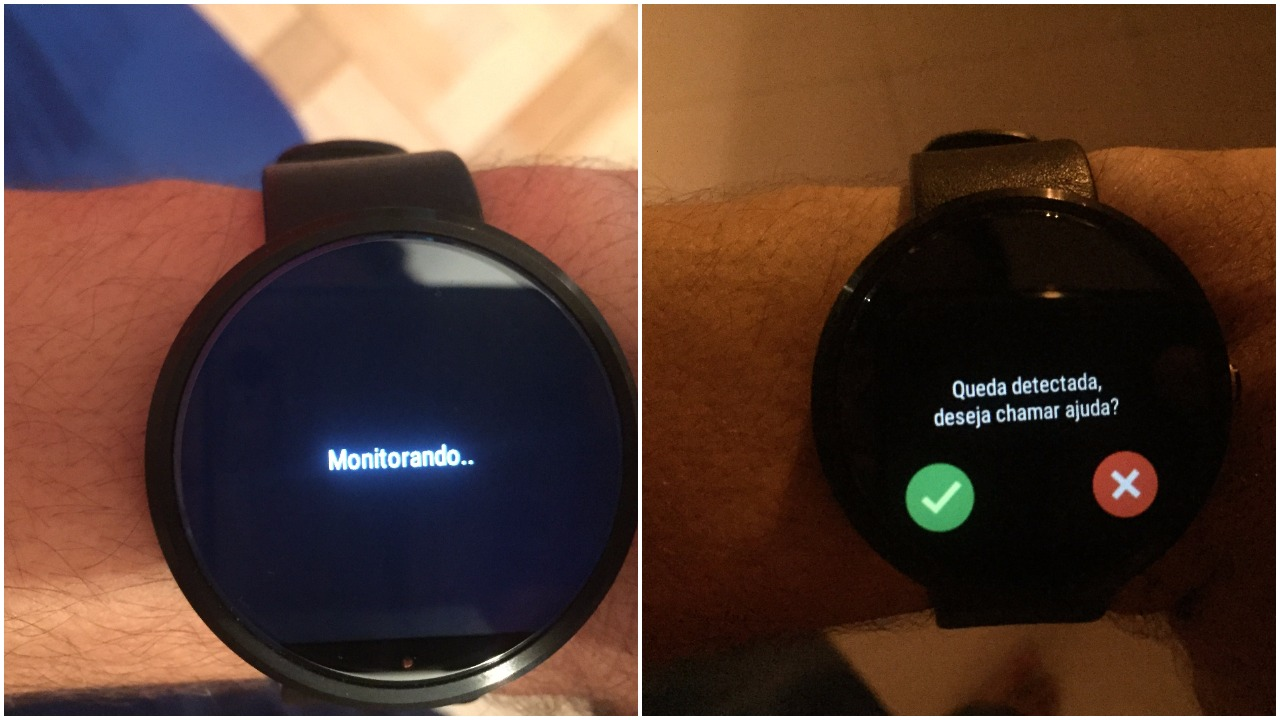
\includegraphics[scale=0.3]{imagens/smartwatch.png}
 	\caption{Na ordem, telas de monitoramento e detecção de quedas. Figura Elaborada pelo autor (2016).}
 	\label{fig:smartwatch_screen}
 \end{figure}
 
 O código fonte no apêndice \ref{ap:algorithm} representa o algoritmo utilizado para realizar a detecção de quedas implementado utilizado a linguagem de programação \textit{JAVA}. 

\subsection{Watch Communicator}
O módulo \textit{Watch Communicator} é responsável pela comunicação entre o smartwatch e o smartphone do usuário. Fisicamente, esta comunicação é realizada via bluetooth, já a nível de software, está comunicação é realizada através do que chamamos na arquitetura Android de \textit{Services}.

No Android, um \textit{Service} é um componente da aplicação capaz de realizar operações de longa duração em segundo plano \cite{servicesAndroidDocs}. No SafeWatch, os \textit{Services} recebem os dados do acelerômetro referentes ao evento de queda, ou seja, todos os registros do acelerômetro 0.4 segundos antes do pico de aceleração, até 2 segundos depois deste valor. Além disso, também é enviado, uma variável booleana indicando se deve-se ou não enviar um e-mail para a lista de contatos de emergência do usuário. Os emails de emergência são enviados para a lista de contato do usuário 15 segundos após um evento de queda, ou antes disso, caso o usuário confirme que precisa de ajuda. 

Para que os contatos da lista de emergência não sejam incomodados desnecessariamente na ocorrência de falsas detecções de quedas, o usuário poderá cancelar o envio dos emails de emergência, dentro de 15 segundos após um evento de queda, caso ele informe que está bem. O tempo de 15 segundos foi escolhido, pois o usuário terá tempo de dar um feedback para o sistema, caso ele não esteja em uma situação de perigo. Da mesma forma, este tempo não irá atrasar o envio da mensagem de emergência quando o usuário realmente precisar. Podemos ver a tela que aparecerá para o usuário em um evento de queda a direita na Figura \ref{fig:smartwatch_screen}. 



\subsection{Fall Handler} 
Este módulo é responsável pelo envio de e-mails e a manipulação de arquivos com os dados de uma queda. Para que se possa realizar o envio de e-mails, foi criado um email padrão do SafeWatch. O envio de e-mail é feito de forma assíncrona, sem bloquear a interação do usuário com a aplicação. O modelo do email pode ser visto na figura \ref{fig:mail_template}. Além de uma mensagem informando que o usuário pode está em uma situação de perigo, um link do \textit{Google Maps}\footnote{https://www.google.com/maps} é anexado com a última localização do usuário obtida pelo sistema.

\begin{figure}[ht]
	\centering
	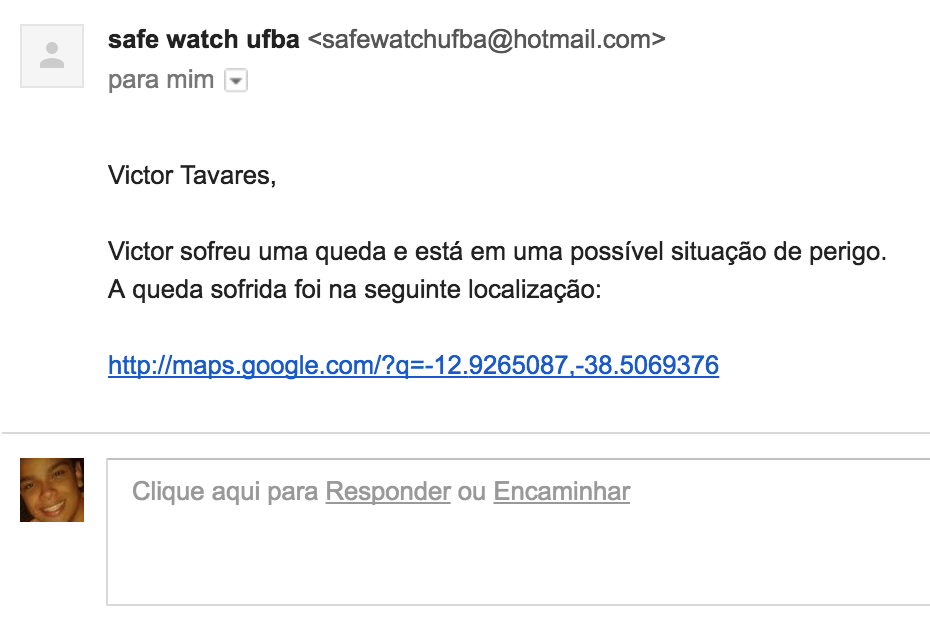
\includegraphics[scale=0.7]{imagens/mail_example.png}
	\caption{ Modelo de email enviado no evento de queda. Figura Elaborada pelo autor (2016).}
	\label{fig:mail_template}
\end{figure}


Os dados referentes a um evento de queda são salvos na raiz do sistema de arquivos do smartphone android na pasta \textit{/SafeWatch/smartwatch}. O arquivo é nomeado com o padrão \textit{experimentData\_timeStamp}, onde t\textit{timeStamp} representa o momento do salvamento do arquivo, em milisegundos. O arquivo está salvo no formato \textit{CSV}, com os valores de aceleração nos eixos x,y,z, o valor de \ac{SMV} correspondente ao registro e o tempo em milisegundos em que ele ocorreu. Apesar destes valores não serem úteis para o usuário final, eles poderão servir para uma possível análise dos dados de queda e replica dos experimentos realizados. 

\subsection{Contact Manager}
Neste módulo, estão encapsuladas as ações de adição, remoção e listagem dos contatos de emergência do usuário. O cadastro dos contatos de emergência deve ser a primeira ação do usuário no primeiro contato com a aplicação. A tela de cadastro e visualização dos contatos de emergência do usuário podem ser vistos na Figura \ref{fig:contacts}. Depois de adicionar os contatos de emergência, o usuário não necessita realizar mais nenhum tipo de cadastro ou configuração no sistema.


\begin{figure}
	\centering
	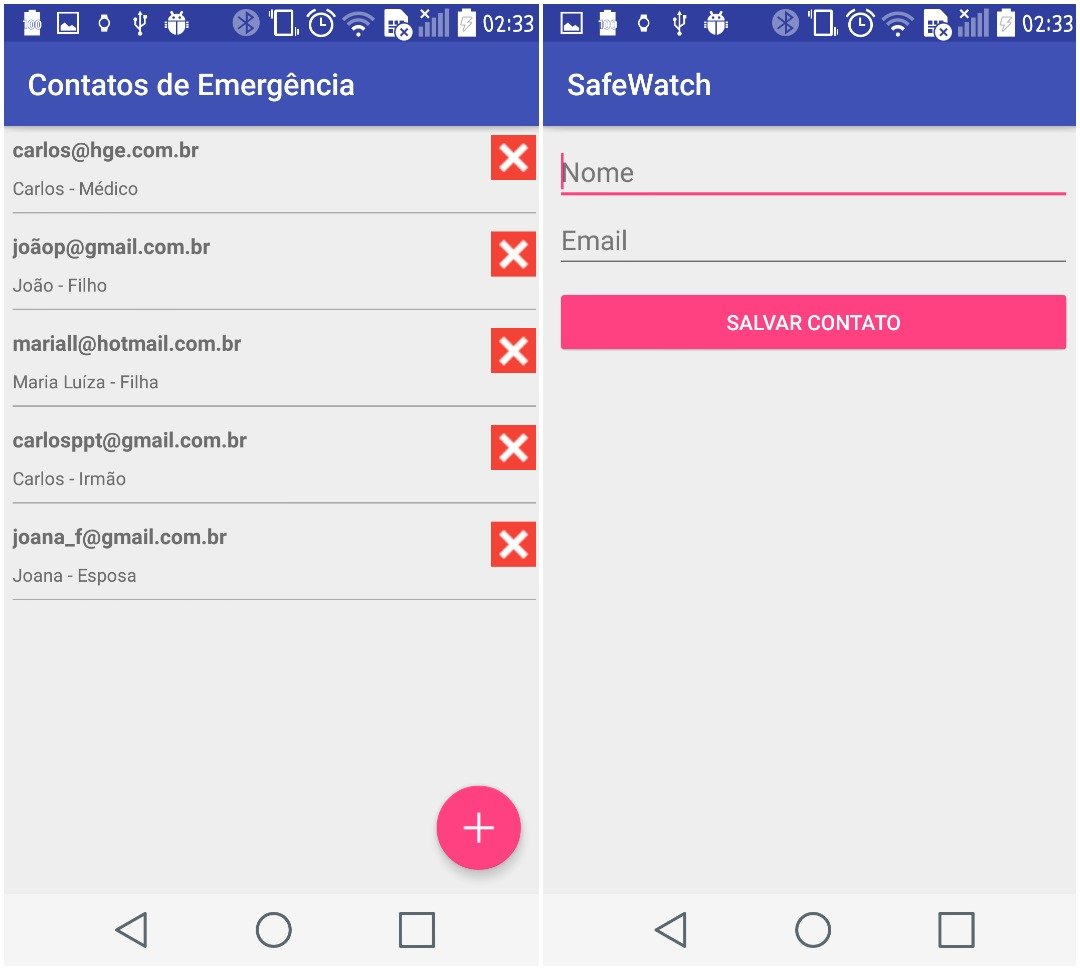
\includegraphics[scale=0.4]{imagens/add_list_contacts.png}
	\caption{Na ordem, telas de listagem e adição de contatos de emergência. Figura Elaborada pelo autor (2016).}
	\label{fig:contacts}
\end{figure}


\section{Sumário}
Neste capítulo foi apresentado uma visão geral do funcionamento do SafeWatch e as principais questões envolvidas no desenvolvimento deste trabalho. Foi descrito em detalhes o algoritmo de detecção de quedas utilizado e as telas presentes nesse sistema.  No próximo capítulo serão descritos detalhes do experimento e as métricas utilizadas na avaliação do SafeWatch. 


